\chapter{\SM}

\section{Las part\'iculas fundamentales y sus interacciones}

Prácticamente todos los datos obtenidos con los experimentos de altas
energías pueden explicarse con el denominado {\SM} de las partículas y sus
interacciones. Esta teoría fue formulada en varios trabajos a partir de la segunda
mitad del siglo XX.

De acuerdo al {\SM} toda la materia esta compuesta por un n\'umero
peque\~no de part\'iculas fundamentales de spin $1/2$, conocidas como fermiones,
que se dividen en dos tipos: quarks y leptones (ver {\tab} \ref{tab:fermions})
Hasta el momento, ningún experimento ha podido encontrar evidencia
de que los fermiones tengan una subestructura interna.

\begin{table}[!ht]
\centering
\begin{tabular}{cccccccccc}
  %%\hline
  %% & Particula & Masa\todo{ref} & Electric Charge & Particle & Mass\todo{ref} & Electric Charge & Particle & Mass\todo{ref} & Electric Charge \\
  \hline \multirow{2}{*}{Leptones} & e & 0.511 \mev & -1 & $\mu$ & 105.7 \mev & -1 & $\tau$  & 1768 \mev & -1 \\
  & $\nu_e$ & $<2.2 \eV$ & 0 & $\nu_\mu$ & $< 0.17 \mev$ & 0 & $\nu_\tau$ & $<15.5 \mev$ & 0 \\
  \hline  \multirow{2}{*}{Quarks} & $u$ & 2.4 \mev & 2/3 & $c$ & 1.27 \gev & 2/3 & $t$ & 171.2 \gev & 2/3 \\
                            & $d$ & 4.8 \mev & -1/3 & $s$ & 104 \mev & -1/3 & $b$  & 4.2 \gev & -1/3 \\
\hline
\end{tabular}
\caption{Partículas fundamentales}\label{tab:fermions}.
\end{table}


La distintas interacciones entre fermiones son descriptas en términos del intercambio de partículas
entre estos. Estas partículas de intercambio son denominadas \emph{bosones}, y a diferencia de los
fermiones tienen spin entero. Los bosones mediadores se muestran en la {\tab} \ref{tab:bosons}.

Existen cuatro tipos de interacciones fundamentales. La interacción fuerte es la responsable
de mantener los quarks formando los protones y neutrones, y es mediada por partículas no masivas
llamadas \emph{gluones}. Las interacciones electromagnéticas son las responsables de todos los
fenómenos extra nucleares, como por ejemplo las fuerzas intermoleculares en líquidos y solidos.
Estas interacciones están mediadas por el intercambio de fotones no masivos.
La interacci\'on débil es la responsable de los procesos de decaimiento $\beta$, y sus mediadores
son los bosones $Z^0$ y $W^\pm$, con masas del orden de 100 veces la masa del protón.
Por ultimo existe una interacción que actúa entre todo tipo de partículas, la interacción gravitatoria.
En la escala de los experimentos de partículas es la interacción mas débil de todas las interacciones
fundamentales, aunque es la dominante en la escala del universo. Es supuestamente mediada por el
intercambio de bosones de spin 2, llamados \emph{gravitones}.

El hecho de que existan cuatro campos de interacciones distintos e independientes es un poco
insatisfactorio y desde Einstein se ha especulado que estas diferentes interacciones sean
distintas manifestaciones de un único campo unificado. En los a\~nos 1970, los experimentos
mostraron que la interacciones débil y electromagnética podían ser unificadas \todo{work here}.

Los leptones interact\'uan de forma d\'ebil y electromagn\'etica en el caso de ser cargados,
o solo d\'ebilmente si son neutros. En contraste, los quarks (que son los constituyentes
fermi\'onicos de los hadrones, y por lo tanto del n\'ucleo at\'omico) interact\'uan adem\'as de
d\'ebil y electromagn\'eticamente, por medio de la interacci\'on fuerte. Esta es la distinci\'on
fundamental entre quarks y leptones.

Las interacciones débil y electromagnética son descriptas de una forma unificada por la
teoría electodebil, que es una generalización de la electrodinámica cuántica (QED), mientras
que la interacción fuerte de los quarks es descripta por la cromodinamica cuántica (QCD), que
también es análoga a QED.

\begin{table}[!ht]
\centering
\begin{tabular}{ccc}
\hline Débil & Electromagnética & Fuerte \\
\hline quarks y leptones & quarks y leptones & quarks \\
\hline $W^+$, $W^-$ y $Z^0$ & $\gamma$ & gluones \\
\hline
\end{tabular}

\caption{Interacciones y los bosones de gauge mediadores de las mismas.}\label{tab:bosons}
\end{table}

%--------------------
% El Modelo Estandar
%--------------------
\section{El \SM}

Formalmente, el {\SM} es una teoría de campos [6, 7, 8] renormalizable [9,10] que provee una descripción
unificada de las interacciones fuerte, débil y electromagnética. Estas interacciones surgen del
requerimiento de que la teoría sea invariante bajo transformaciones de gauge locales del grupo
de simetría

%% Formalmente, el {\SM} es una teoria de gauge no abeliana, construida imponiendo invarianza de gauge
%% local sobre los campos cuentificados que describen las particulas fundamentales, dando lugar a los
%% campos de gauge que describen las interacciones. Su grupo de simetria es,

\begin{equation}
  \text{SU}(3)_C \times \text{SU}(2)_L \times \text{U}(1)_Y
\end{equation}
%
donde $Y$, la hipercarga, $L$, la helicidad izquierda, y $C$, la carga de color, representan
kas cantidades conservadas del grupo de simetría. El subgrupo $\text{SU}(2)_L \times \text{U}(1)_Y$
representa el sector electrodébil, es decir, la electrodinámica cuántica mas las interacciones
débiles. Y la adición del grupo $\text{SU}(3)_C$ incluye la cromodinamica cuántica

%% La cromodinamica cuantica es la teoria de campos de gauge que describe las interacciones
%% fuertes de los quarks y gluones que poseen carga de color. Es la componente SU(3) del
%% $\text{SU}(3) \times \text{SU}(2) \times \text{U}(1)$ del \SM.

La masa de las part\'iculas en el {\SM} puede ser introducida mediante el llamado mecanismo
de Higgs\cite{PhysRevLett.13.321, PhysRevLett.13.508}, vía la ruptura espontánea de la simetría
electrodébil.

\begin{equation}
  \text{SU}(3)_C \times \text{SU}(2)_L \times \text{U}(1)_Y \to \text{SU}(3)_C \times \text{U}(1)_Q
\end{equation}
%
que resulta en la generación de los bosones de guage masivos $W^\pm$ y $Z$. Como consecunecia de esto,
ademas, un nuevo campo escalar debe ser agregado al Lagrangiano, dando lugar a la
aparici\'on de un nuevo boson masivo, $H$, de spin 0, al que se lo llam\'o \emph{bos\'on de Higgs}.

Weinberg y Salam fueron los primeros en aplicar el mecanismo de Higgs al rompimiento de la
simetria electrodebil [6,7] y mostraron como este mecanismo podia ser incorporado a la teoria
electroweak de Glashow [8], dando inicios a lo que hoy conocemos como {\SM} de la fisica
de particulas.

La relacion entre las masas de los bosones $W^\pm$ y $Z$ predicha por el {\SM} esta dada por

\begin{equation}
  \frac{m_W}{m_Z} = \cos \theta_W
\end{equation}
%
donde $\theta_W$ es el angulo de mezcla de Weinberg, relaciona las constantes de acoplamiento
debil ($g$) con la electromagnetica ($g'$) como  $\tan\theta_W = g'/g$.
Los bosones $W^\pm$ y $Z$ fueron descubiertos en 1982 por las colaboraciones UA1 y UA2 del
experimento SppS del CERN \todo{Agregar referencia}.

No solo los bosones de guage adquieren masa debido al mecanismo de Higgs, tambien lo hacen
los fermiones que forman la materia. El descubirmiento del quark top en 1995 por las colaboraciones
D0 y CDF...

%% El último componente del Modelo Estándar es el mecanismo de Higgs que permite que el MS sea una teoría
%% matemáticamente consistente de partículas fundamentales con masa. Éste postula la existencia de un bosón
%% de spin 0, el bosón de Higgs. En la siguiente sección se describirá este mecanismo.

%% Todas las observaciones experimentales son compatibles con el Modelo Estándar a un nivel de muy alta precisión,
%% aunque no todos los componentes del modélo han sido comprobados experimentalmente. En particular, el mecanismo
%% de Higgs por el cual las partículas fundamentales adquieren masa, necesita todavía de su verificación experimental.
%% Además, aunque todos los componentes sean establecidos experimentalmente en el futuro, el modelo no puede
%% considerarse como la teoría definitiva para la materia y las interacciones. Las simetrías y los parámetros
%% fundamentales (masas y constantes de acoplamiento) no pueden ser derivadas. Y la fuerza de gravedad no puede
%% incorporarse de la misma forma que las otras interacciones.

%% El {\SM} es un conjunto de teorías de gauge, y necesita tres simetrías internas para describir las
%% partículas y sus interacciones. El grupo de simetría del modelo estándar es $SU(3) \times SU(2) \times U(1)$.

%% Todos los resultados de experimentos son consistentes con la noción de que estas tres simetrías son
%% necesarias y suficientes para describir las interacciones de las partículas conocidas. Las
%% interacciones de los campos de fuerzas y las partículas que forman la materia son descriptas por
%% teorías de gauge abelianas y no abelianas en este grupo de simetría. La simetría $SU(3)$ está
%% asociada a la interacción fuerte, y el bosón de intercambio es el gluón, que es no masivo.
%% Cualquier partícula que se transforme con respecto a esta simetría se dice que tiene carga de color,
%% e interacciona fuertemente. La interacción electrodébil está asociada a los términos $SU(2) \times U(1)$,
%% e involucra a los bosones $W^+$, $W^-$, $Z^0$ y al fotón.

%% Los leptones son, por definición, aquellos que no experimentan la interacción fuerte, es decir no llevan carga
%% de color pero tienen asociada una carga electrodébil.
%% Los \emph{quarks} por otro lado, experimentan las tres interacciones fundamentales del MS.

%% Como se mencionó, además de la interacción fuerte, débil y electromagnética entre \emph{quarks} y leptones,
%% existe una cuarta fuerza en la naturaleza, la gravedad. Sin embargo, la interacción gravitatoria entre partículas
%% elementales es tan débil, que puede ser despreciada a las energías accesibles hasta el momento. Por el momento
%% la gravedad no puede ser incluída en el MS porque no existe una teoría de campo cuántica de la gravedad.




%% Actualmente la teoría que explica a los constituyentes fundamentales de la materia y sus
%% interacciones es conocida como {\SM} (SM, de sus siglas en inglés)\cite{martinshaw}\cite{gordonkane}\cite{burguesmoore}.
%% Existe un grupo pequeño de partículas fundamentales, de dos grupos distintos: los constituyentes de la materia, dos grupos de fermiones de spin $\frac{1}{2}$, formados por seis leptones y seis quarks, y los bosones de spin 1, llamados bosones de gauge, que son los mediadores de las fuerzas en la teoría (electromagnética, débil y fuerte). Los leptones y quarks a su vez se encuentran divididos en tres familias cada uno de idéntica estructura. Todas las partículas del modelo estándar se suponen elementales, es decir, son tratadas como partículas puntuales, sin estructura interna ni estados excitados.
%% En la tabla \ref{tab:quarksleptones} se resumen los constituyente fundamentales de la materia.


%% \section{El mecanismo de Higgs}

%% El mecanismo de Higgs es una de las ultimas piezas que componen el {\SM}. %% , en este sector de la teoría, campos
%% %% escalares interactúan de manera tal que el estado fundamental adquiere un valor de expectación no
%% %% nulo, rompiendo espontáneamente la simetría electrodébil.

%% %mandl-sahw
%% El bosón de Higgs es una partícula de spin 0 cuya existencia es predicha por el mecanismo de
%% Higgs\cite{mandlshaw}, pero no habia sido observado hasta el momento.
%% La invariancia de gauge debida a la simetría $SU(3) \times SU(2) \times U(1)$ impide que haya
%% partículas masivas. Por otro lado, el agregado \emph{ad hoc} de términos de masa en el
%% lagrangiano anula la invarianza del mismo. Para poder obtener una teoría renormalizable,
%% es necesario introducir las masas por un mecanismo que mantenga la invarianza del lagrangiano.

%% Sin embargo, el problema es resuelto por el mecanismo de Higgs, donde las masas son introducidas
%% de una manera consistente mediante el proceso de ruptura espontánea de simetría.
%% La simetría $SU(2)_L \times U(1)$ es espontáneamente rota en $U(1)_{em}$ dando lugar a la presencia
%% de tres bosones de gauge masivos ($Z^0$, $W^{\pm}$) y un único no masivo ($\gamma$), a costo de
%% un nuevo grado de libertad, el campo de Higgs.

%% Para poder entender lo que se conoce como ruptura espontánea de simetría,
%% consideremos un lagrangiano que posee una simetría particular, es decir, es invariante frente
%% a las transformaciones de simetría correspondientes. Al clasificar los niveles de energía del
%% sistema, dos situaciones pueden ocurrir. Primero, si un estado de energía es no degenerado,
%% el correspondiente estado es único e invariante bajo esa simetría del lagrangiano.
%% En segundo lugar, puede ocurrir que el nivel de energía esté degenerado y sus correspondientes
%% estados no sean invariantes pero se transformen linealmente entre ellos mismos bajo las
%% transformaciones de simetría de $\mathcal{L}$. En particular, consideremos el estado más bajo
%% del sistema. Si no es degenerado, el estado de más baja energía es único y posee las simetrías
%% de $\mathcal{L}$. En el segundo caso, si está degenerado, no hay un único estado que represente
%% ese estado fundamental. Si arbitrariamente elegimos uno de esos estados degenerados como el
%% estado fundamental, este no compartirá más las simetrías con $\mathcal{L}$. Esta forma de obtener
%% un estado fundamental que tenga la simetría de $\mathcal{L}$, se conoce como ruptura espontánea
%% de simetría.


%% \subsection{El modelo de Goldstone}

%% El modelo de Goldstone es un modelo simple con ruptura espontánea de simetría. Comenzando con una teoría clásica, se toma la densidad lagrangiana:

%% \begin{equation}
%% \mathcal{L}= \partial^{\mu}\phi^*(x)\partial_{\mu}\phi(x)-V(\phi) \label{eq:1}
%% \end{equation}

%% con $\phi(x)$ un campo complejo
%% \begin{equation}
%% \phi(x)= \frac{\sqrt{2}}{2}[\phi_1(x)+\phi_2(x)]\label{eq:2}
%% \end{equation}
%% y $V(\phi)$ la energía potencial de la forma:

%% \begin{equation}
%% V(\phi)=\mu^2 |\phi(x)|^2 + \lambda |\phi(x)|^4\label{eq:3}
%% \end{equation}

%% Las constantes $\mu^2$, $\lambda$ son reales con $\lambda$ positiva de forma que la energía total del campo tenga una cota inferior. Esta densidad lagrangiana es invariante frente a transformaciones globales $U(1)$ que describen rotaciones en el plano complejo. \\
%% Exigiendo que el estado de menor energía (vacío), sea invariante frente a transformaciones de Lorentz y traslaciones, implica que $\phi(x)$ es una constante en este estado. Dependiendo del valor de $\mu^2$ existen dos posibilidades para el estado vacío. Si $\mu^2$ es positivo, la situación es normal con el mínimo del potencial cuando $\phi=0$. Si, en cambio, $\mu^2$ es negativo el mínimo de la energía no corresponde a un único valor de $\phi$ sino que esta degenerado, siendo el mínimo un anillo en el plano complejo

%% \begin{equation}
%% \phi_{Vmin}=\sqrt{\frac{-\mu^2}{2\lambda}}e^{i\theta}\label{eq:4}
%% \end{equation}
%% Dado que la densidad lagrangiana \ref{eq:1} es invariante frente a rotaciones en el plano complejo de $\phi$ cualquier dirección es igualmente válida. Se tomará en particular, $\theta=0$ quedando

%% \begin{equation}
%% \phi_{Vmin}=\sqrt{\frac{-\mu^2}{2\lambda}}=\upsilon/\sqrt{2}\label{eq:5}
%% \end{equation}

%% Una teoría donde el estado vacío tiene menos simetría que la densidad lagrangiana es llamada una teoría con ruptura espontánea de simetría. Podemos representar a $\phi$ de la siguiente manera
%% \begin{equation}
%% \phi(x)=\frac{\sqrt{2}}{2}[\upsilon+\sigma(x)+i\eta(x)]\label{eq:6}
%% \end{equation}
%% donde $\sigma(x)$ y $\eta(x)$ representan las desviaciones respecto del valor mínimo elegido. La densidad lagrangiana \ref{eq:1} reescrita en términos de $\sigma(x)$ y $\eta(x)$ es

%% \begin{eqnarray}
%% \mathcal{L}= \frac{1}{2}\partial^{\mu}\sigma(x)\partial_{\mu}\sigma(x)-\lambda\upsilon^2\sigma(x)^2+ \frac{1}{2}\partial^{\mu}\eta(x)\partial_{\mu}\eta(x) -\nonumber \\
%% - \lambda\upsilon\sigma(x)[\sigma(x)^2+\eta(x)^2]-\frac{1}{4} \lambda[\sigma(x)^2+\eta(x)^2]\label{eq:7}
%% \end{eqnarray}
%% donde se suprimieron los términos constantes. Tomando los términos de mayor orden como interacciones, la densidad lagrangiana libre toma la forma
%% \begin{equation}
%% \mathcal{L}= \frac{1}{2}\partial^{\mu}\sigma(x)\partial_{\mu}\sigma(x)-\lambda\upsilon^2\sigma(x)^2+ \frac{1}{2}\partial^{\mu}\eta(x)\partial_{\mu}\eta(x)\label{eq:8}
%% \end{equation}

%% Se ve que $\sigma$ y $\eta$ son dos campos de Klein-Gordon reales. Cuantificando los mismos, la densidad lagrangiana \ref{eq:8} describe dos partículas diferentes de spin 0. Los bosones $\sigma$ tendrán masa de valor
%% \begin{equation}
%% m_{\sigma}=\upsilon\sqrt{2\lambda} \label{eq:9}
%% \end{equation}
%% que sale del término que contiene $\sigma^2$, mientras que los bosones $\eta$ tendrán masa nula (como consecuencia directa de la degeneración del mínimo de la energía). Los términos restantes de \ref{eq:7} pueden ser tratados como interacciones entre las partículas $\sigma$ y $\eta$ usando teoría de perturbaciones.

%% Vemos entonces que a partir de la ruptura espontánea de la simetría $U(1)$ global, se obtiene una teoría perturbativa con un boson escalar masivo.


%% \subsection{El mecanismo de Higgs}

%% Lo que se conoce como el mecanismo de Higgs es la extensión del rompimiento espontáneo de simetría para crear un bosón vectorial masivo en una teoría invariante de gauge. Trataremos el caso de una teoría invariante frente a $U(1)$. La idea es entonces reemplazar la derivada normal de \ref{eq:1} por la derivada covariante

%% \begin{equation}
%% D_{\mu}=\partial_{\mu}+iqA_{\mu}\label{eq:10}
%% \end{equation}

%% Agregando además, el término que corresponde al campo de gauge $A_{\mu}$ libre, se tiene
%% \begin{equation}
%% \mathcal{L}= D^{\mu}\phi^*(x)D_{\mu}\phi(x)-V(\phi)-\frac{1}{4} F_{\mu\nu}F^{\mu\nu}\label{eq:11}
%% \end{equation}
%% Esta nueva densidad lagrangiana es invariante frente a transformaciones de gauge $U(1)$ de la forma
%% \begin{eqnarray}
%% \phi(x)\rightarrow \phi'(x)=\phi(x)\, e^{iq\xi(x)} \nonumber \\
%% A_{\mu}\rightarrow A_{\mu}'(x)=A_{\mu}(x) + \partial_{\mu}\xi(x)\label{eq:12}
%% \end{eqnarray}
%% con $\xi(x)$ una función real diferenciable cualquiera. Continuando de la misma manera que para el modelo de Goldstone con un $\mu^2$ negativo, y expresando la densidad lagrangiana en términos de las variables $\sigma(x)$ y $\eta(x)$ definidas en \ref{eq:6} se tiene que
%% \begin{eqnarray}
%% \mathcal{L}=\frac{1}{2}\partial^{\mu}\sigma(x)\partial_{\mu}\sigma(x)-\lambda\upsilon^2\sigma(x)^2 + \frac{1}{2}\partial^{\mu}\eta(x)\partial_{\mu}\eta(x) -\frac{1}{4} F_{\mu\nu}F^{\mu\nu} + \nonumber \\
%% +\frac{1}{2}q^2\upsilon^2A_{\mu}A^{\mu}+ q\upsilon A^{\mu}\partial_{\mu} \eta + \text{términos de orden superior}\label{eq:13}
%% \end{eqnarray}
%% La densidad lagrangiana tiene claramente un bosón vectorial masivo A y dos campos escalares $\sigma$ y $\eta$, con $\eta$ de masa nula; pero desafortunadamente también un término de la forma $A^{\mu}\partial_{\mu}\eta$ que no es posible ajustar. No puede ser interpretado como una interacción perturbativa, ya que es cuadrático en los campos al igual que para los campos libres. Sin embargo, un análisis cuidadoso muestra que la densidad lagrangiana \ref{eq:13} tiene un grado de libertad de sobra. Este grado de libertad extra puede ser absorbido eligiendo un gauge específico, de modo de eliminar $\eta$. Este tipo de transformaciones es siempre posible y para este caso se conoce como gauge unitario. La densidad lagrangiana resultante luego de esta transformación es

%% \begin{eqnarray}
%% \mathcal{L}= \frac{1}{2}\partial^{\mu}\sigma(x)\partial_{\mu}\sigma(x)- \lambda\upsilon^2\sigma(x)^2 - \frac{1}{4} F_{\mu\nu}F^{\mu\nu} + \frac{1}{2} q^2\upsilon^2A_{\mu}A^{\mu} + \nonumber \\
%% + \text{términos de orden superior}\label{eq:14}
%% \end{eqnarray}

%% Resumiendo, se puede ver que un campo complejo escalar y un campo vectorial de masa nula, ambos con dos grados internos de libertad, fueron transformados en un campo real escalar, con un solo grado de libertad, y un bosón vectorial masivo, con tres grados de libertad, como resultado del mecanismo de Higgs. \\

%% El mecanismo de Higgs fue mostrado aquí para una teoría invariante frente a transformaciones de gauge $U(1)$. Para extender el mismo a teorías invariantes frente a $SU(2)\times U(1)$ como la electro-débil se comienza con una densidad lagrangiana con un doblete escalar complejo y cuatro bosones vectoriales sin masa, es decir, con un total de 12 grados internos de libertad.
%% Mediante el mecanismo de Higgs, la densidad lagrangiana se transforma en un campo real escalar, tres bosones vectoriales masivos y un boson vectorial de masa nula. Este último es, por supuesto, identificado como el fotón, mientras que el cuanto del campo escalar es el bosón de Higgs. \\

%La introducción de las masas a los bosones de intercambio con un doblete escalar complejo, es el camino mas simple, ya que en principio un número infinito de campos escalares pueden ser introducidos. Los modelos supersimétricos mas simples obtienen cinco campos escalares luego del mecanismo de Higgs: un doblete cargado escalar, dos escalares neutros y un pseudoescalar neutro.


Desde el punto de vista teórico la masa del bosón de Higgs es un parámetro
libre dentro del {\SM} y por lo tanto ninguna predicción puede ser hecha.

La b\'usqueda del boson de higgs, la unica particula del {\SM} que
no habia sido descrubierta aun, fue uno de los grandes objetivos por los
cuales se dise\~no y construyó el Gran Colisionar de Hadrones (LHC).

%% Existian limites indirectos a la masa del Higgs
%% Indirect limits on the SM Higgs boson mass of mH <
%% 158 GeV at 95% confidence level (CL) have been set
%% using global fits to precision electroweak results \cite{ALEPH:2010aa}.
%% Direct searches at LEP [13], the Tevatron [14–16] and
%% the LHC [17, 18] have previously excluded, at 95% CL,
%% a SM Higgs boson with mass below 600 GeV, apart from
%% some mass regions between 116 GeV and 127 GeV.

En el a\~no 2012 el CERN anuncio el descubrimiento de una particula
consistente con el boson de Higgs por parte de los dos grandes
experimentos del LHC, ATLAS y CMS \cite{Aad:2012tfa,Chatrchyan:2012ufa}.

La masa $m_H$ del boson de Higgs no es predicha por la teoria. Sin embargo,
algunas cosideraciones generales muestran que debe ser menor a 1 TeV, y
algunas medidas de precision electrodebiles implican que $m_H < 152 \gev$ a
95\% de nivel de confianza (CL).

\begin{figure}[!ht]
  \centering
  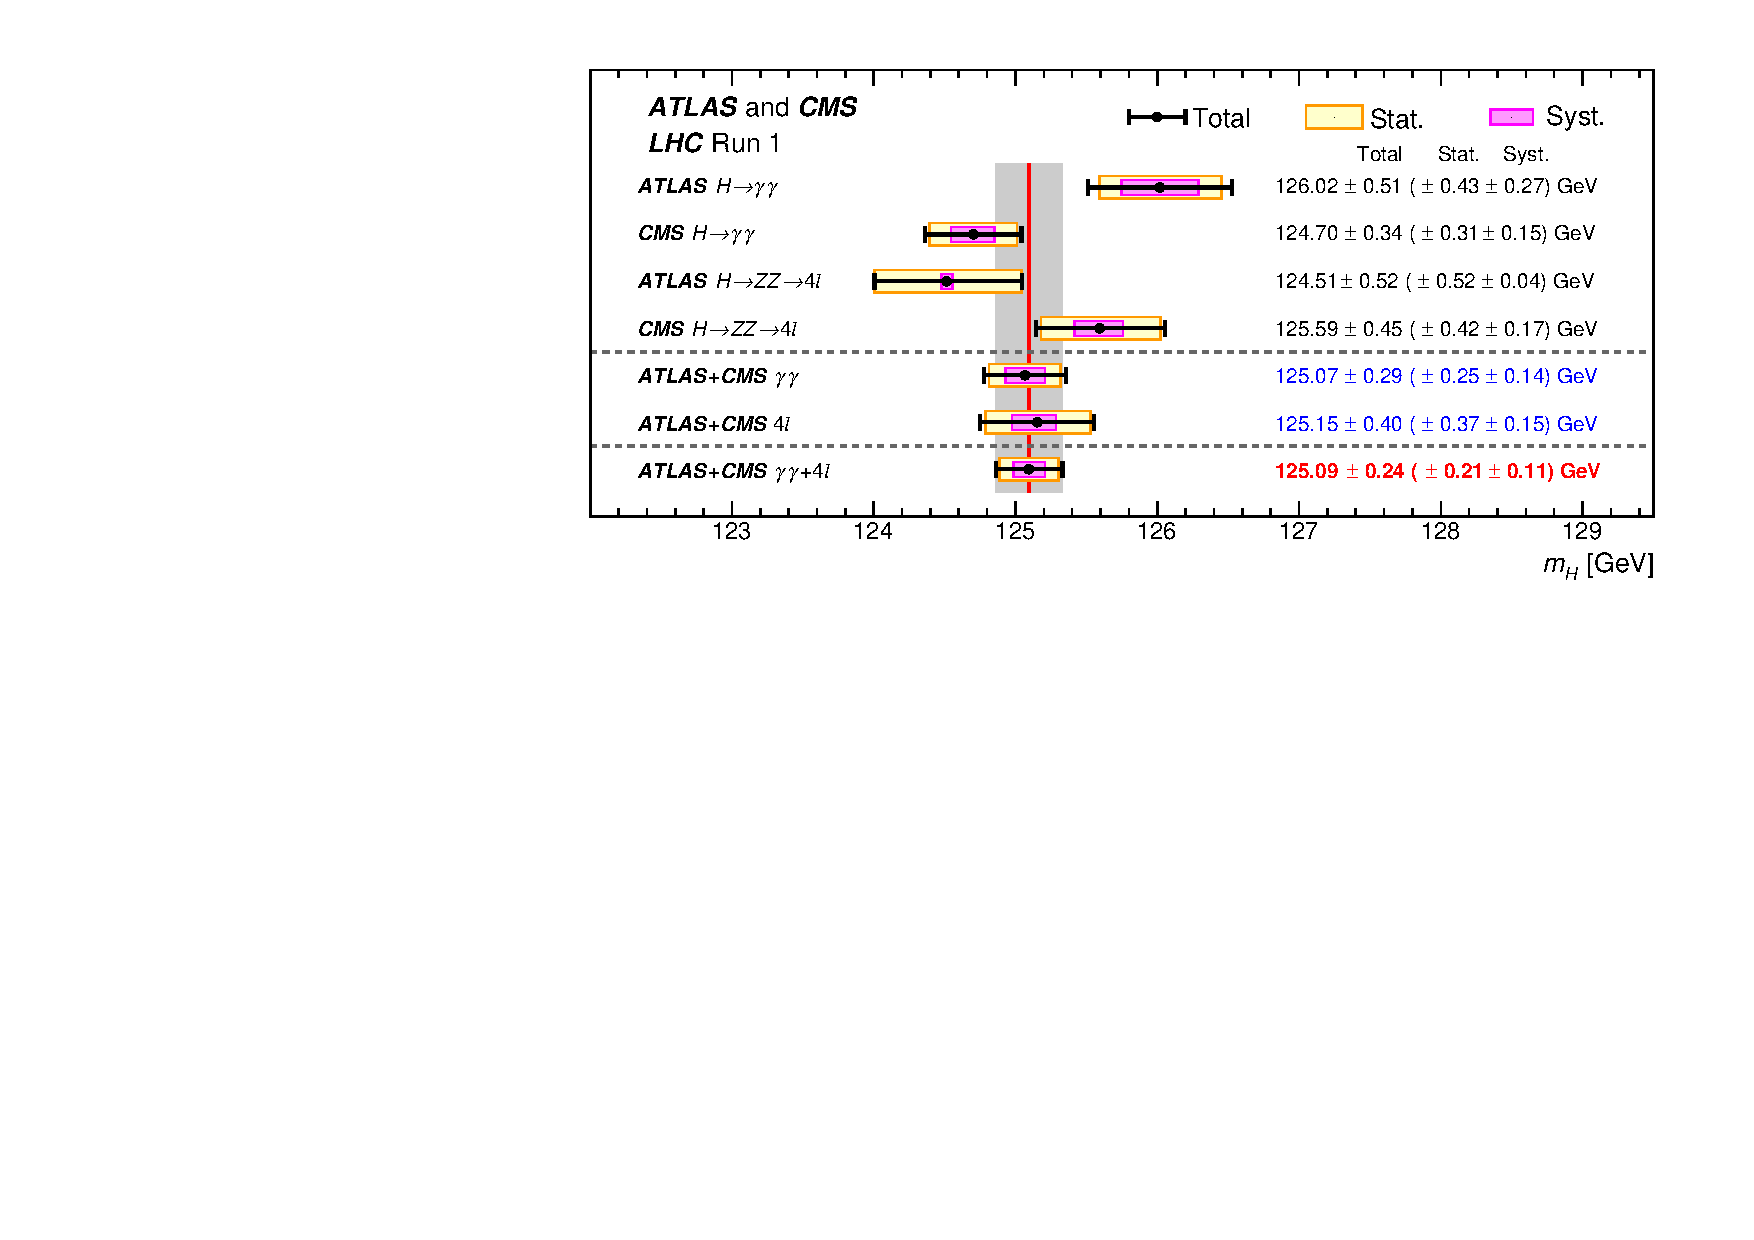
\includegraphics[width=0.8\textwidth]{figures/higgs_atlas_cms_mass}

  \includegraphics[width=0.8\textwidth]{figures/higgs_atlas_cms_bestfit}
  \caption{Caption}
  \label{fig:higgs_cms_atlas}
\end{figure}

%% Durante los pasados veinte a\~nos se han llevado a cabo busquedas
%% directas del boson de Higgs en el colisionador LEP, dejando un
%% limite inferior para la masa $m_H > 114.4 \gev$

%% Over the past twenty years, direct searches for the Higgs
%% boson have been carried out at the LEP collider, leading to a lower
%% bound of m H > 114 . 4 GeV at 95% CL [15], and at the Tevatron
%% proton–antiproton collider, excluding the mass range 162–166 GeV
%% at 95\% CL [16] and detecting an excess of events, recently reported
%% in [17–19], in the range 120–135 GeV.




%% Por otro lado, se supone comúnmente que el MS es simplemente una teoría efectiva a bajas energías de alguna teoría mas fundamental que explique el origen de la ruptura de la simetría electrodébil.
%% Por esto deberá existir alguna escala de energía $\Lambda$ a la que el modelo deje de funcionar. Es decir, el Modelo Estándar no sería mas adecuado para describir la teoría por encima de $\Lambda$
%% y grados de libertad relativos a la nueva física se hacen relevantes. Aunque, el valor de $\Lambda$ es desconocido, para un dado valor se puede calcular el valor mínimo y máximo permitidos para
%% la masa del bosón de Higgs basados en argumentos teóricos. En la Figura \ref{fig:masahiggs} se pueden ver estos limites en función de la escala $\Lambda$, donde la región permitida esta delimitada
%% por dos curvas. La región de masas 130 GeV $< m_H <$180 GeV sería consistente con la hipótesis $\Lambda= M_{pl}$, esto significaría que el MS seria válido en principio hasta la escala de Planck.
%% Por el contrario si la masa del bosón de Higgs está fuera de ese rango, significaría que la escala sería $\Lambda < M_{pl}$ y algunas evidencia de nueva física deberían encontrase próximamente.

La {\fig} \ref{fig:sm_atlas_xs} muestra el buen acuerdo entre la sección eficaz de algunos
procesos del {\SM} medidas por ATLAS\todo{Agregar refencia del plot} y las predicciones
teóricas.

\begin{figure}[h]
  \centering
  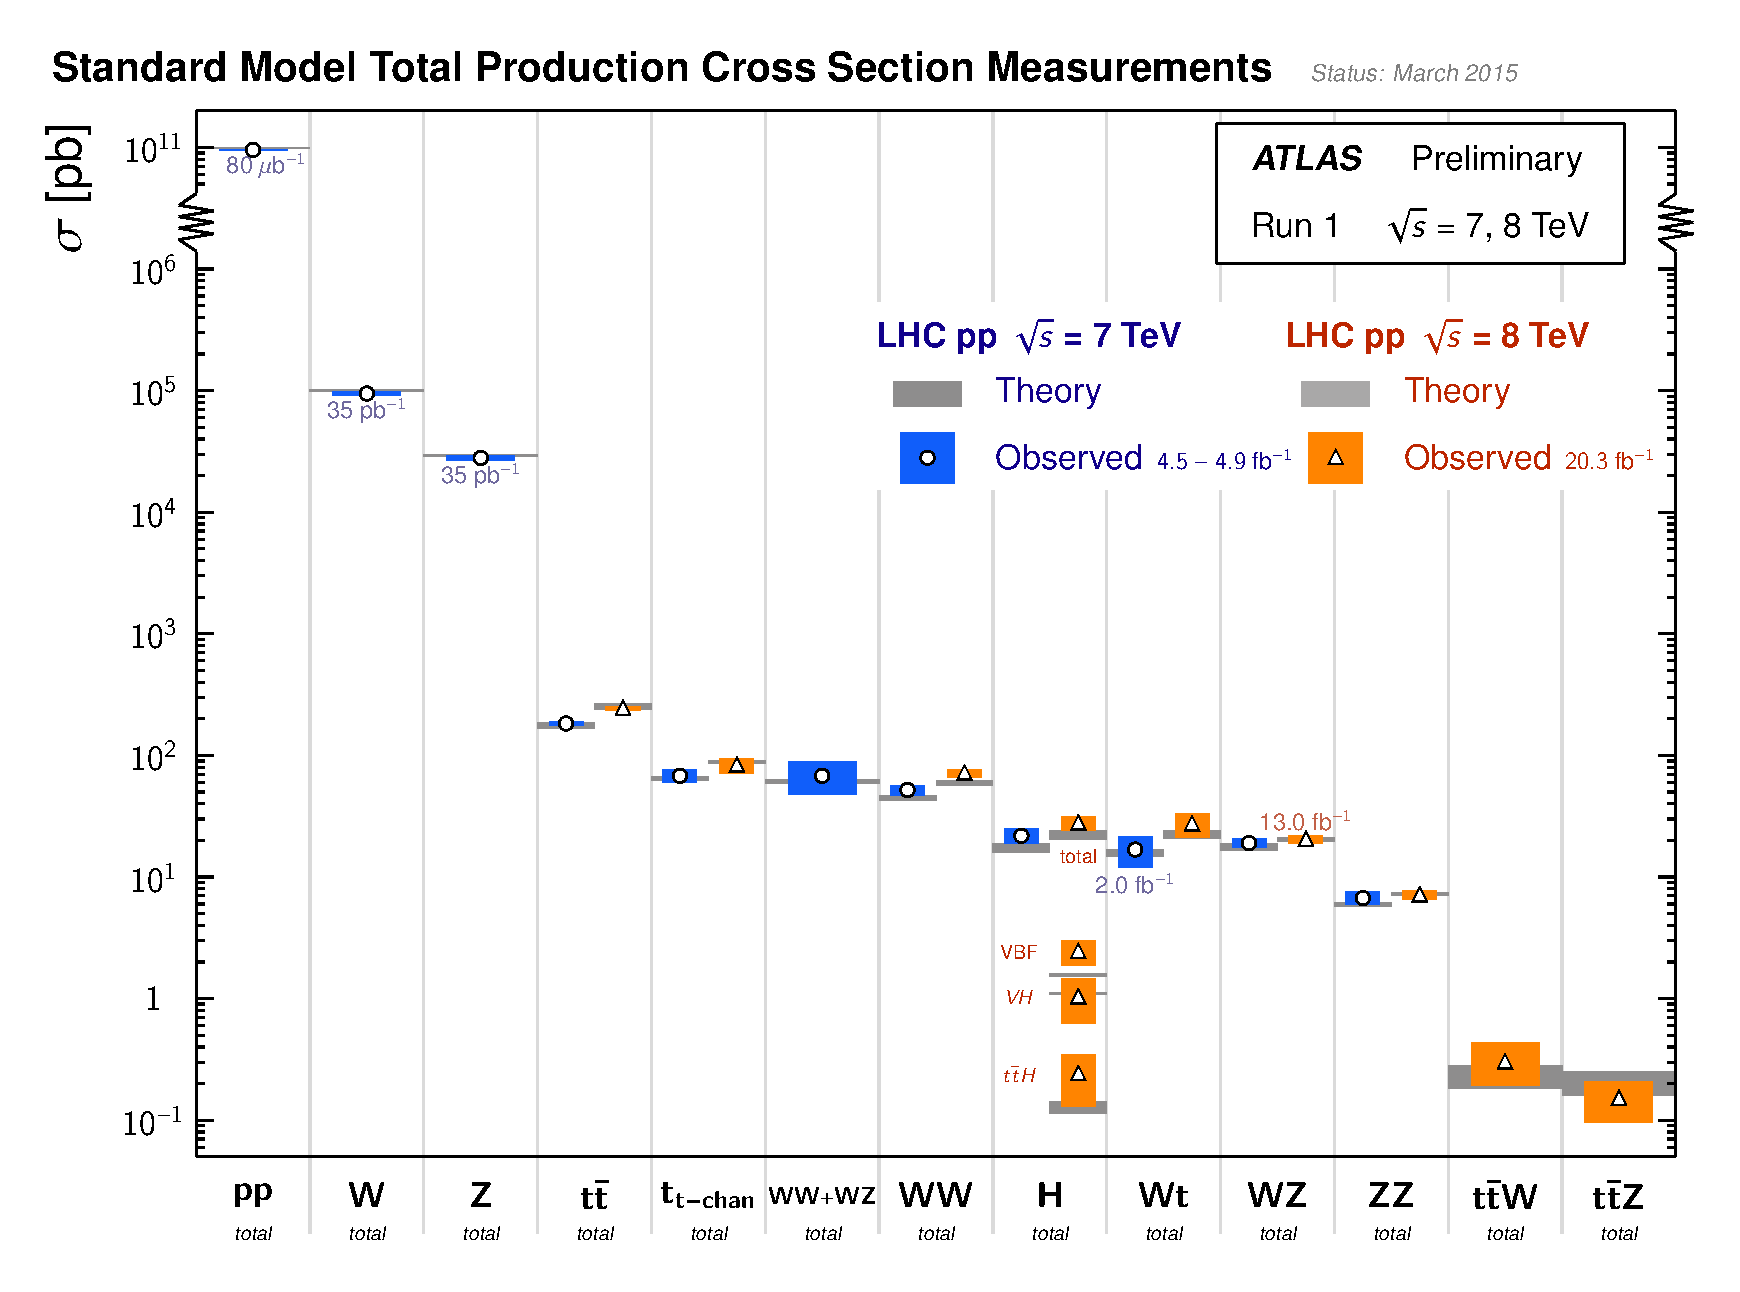
\includegraphics[width=1\textwidth]{figures/ATLAS_a_SMSummary_TotalXsect.pdf}
  \caption{Resumen de las distintas medidas de secci\'on eficaz de producci\'on de muchos
    procesos del {\SM}, comparadas con sus valores teoricos esperados.
    Los valores teoricos esperados fueron calculados como minimo a NLO.
  }\label{fig:sm_atlas_xs}
    %% Summary of several Standard Model total production cross section measurements,
    %% corrected for leptonic branching fractions, compared to the corresponding theoretical
    %% expectations. All theoretical expectations were calculated at NLO or higher. The W and Z
    %% vector-boson inclusive cross sections were measured with 35 pb-1 of integrated luminosity
    %% from the 2010 dataset. All other measurements were performed using the 2011 dataset or the
    %% 2012 dataset. The luminosity used for each measurement is indicated close to the data point.
    %% Uncertainties for the theoretical predictions are quoted from the original ATLAS papers.
    %% They were not always evaluated using the same prescriptions for PDFs and scales. }
\end{figure}


%% \section{Debilidades del {\SM}}
\section{Física más alla del {\SM}}

A pesar de todo lo dicho anteriormente el {\SM} sufre de algunas debilidades. Algunas del
punto de vista teorico, mientras que otras de algunas mediciones experimentales que no pueden
acomodarse dentro del modelo.


% neutrino mass
Los neutrinos tienen masas muy peque\~nas comparadas con los demas fermiones. Solo se tienen
limites superiores para estas (ver {\tab} \ref{tab:fermions}).

El termino de masa para fermiones puede escribirse usando el doblete de Higgs si existen
los fermiones de helicidad izquierda y derecha para un dado sabor. La masa obtenida por
esta interacci\'on es llamada masa de Dirac. Para que este mecanismo puede ser utilizado
en los neutrinos, deberian exixste los neutrinos de helicidad derecha. Aunque todavia
no entendemos porque existen los fermiones de helicidad derecha pero no para los nuetrinos.

En el {\SM} los neutrinos son particulas sin masa.

\begin{itemize}\itemsep0.2cm\parskip0.2cm
\item  dark energy and dark matter

\item gravity

\item hierarchy
\end{itemize}
